% Created 2016-08-17 Wed 14:38
\documentclass[tikz,convert]{standalone}
\usepackage[utf8]{inputenc}
\usepackage[T1]{fontenc}
\usepackage{tikz}
\usetikzlibrary{calc}
\usetikzlibrary{arrows}

\author{Holger Karl}
\date{\today}
\title{}
\begin{document}

% normale Zuweisung: 
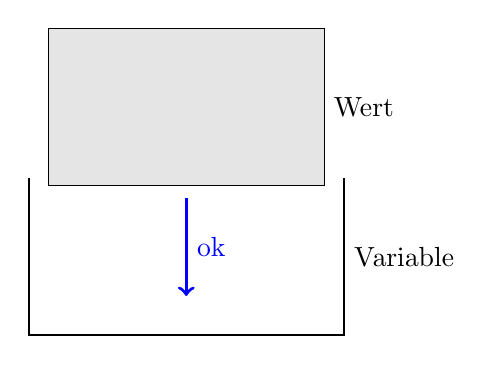
\begin{tikzpicture}
  \draw [thick] (0,0) -- (0, -2) -- (4,-2) -- (4, 0) node [right, midway] {Variable};
  \filldraw [fill=gray!20] (0.25,2-0.1) -- (0.25, 0-0.1) -- (4-0.25, 0-0.1) -- (4-0.25, 2-0.1)
node [right, midway] {Wert} -- (0.25,2-0.1) ;
  \draw [->, very thick, blue] (2,-0.25) -- (2,-1.5) node [right, midway, blue] {ok};
\end{tikzpicture}

% Kreis an Box: 
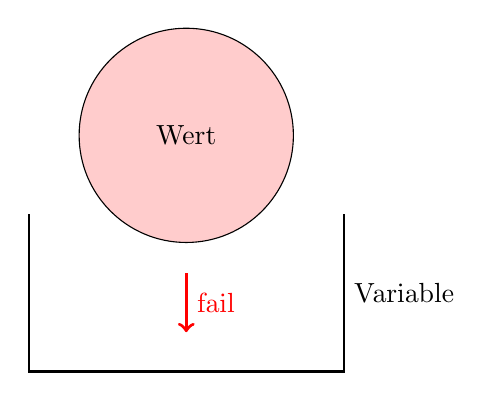
\begin{tikzpicture}
  \draw [thick] (0,0) -- (0, -2) -- (4,-2) -- (4, 0) node [right, midway] {Variable};
  \path (2,1)  node [shape=circle, draw, fill=red!20, inner sep = 20] {Wert};
  \draw [->, very thick, red] (2,-0.75) -- (2,-1.5) node [right, midway, red] {fail};
\end{tikzpicture}

% Kreis und Typecasting 
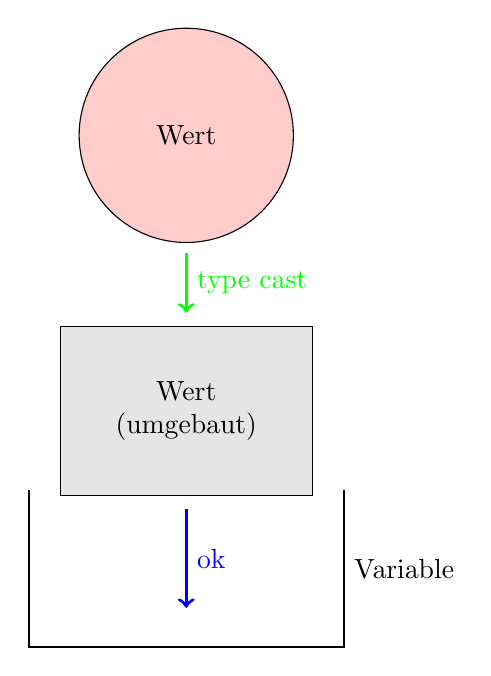
\begin{tikzpicture}
  \draw [thick] (0,0) -- (0, -2) -- (4,-2) -- (4, 0) node [right, midway] {Variable};
  \path (2,4.5)  node [shape=circle, draw, fill=red!20, inner sep = 20] {Wert};
  \draw [->, very thick, green] (2,3) -- (2,2.25) node [right, midway, green] {type cast};
  \path (2,1)  node [shape=rectangle, draw, fill=gray!20, inner sep = 20,align=center] {Wert\\ (umgebaut)};
  \draw [->, very thick, blue] (2,-0.25) -- (2,-1.5) node [right, midway, blue] {ok};
\end{tikzpicture}

% Inhertiance 
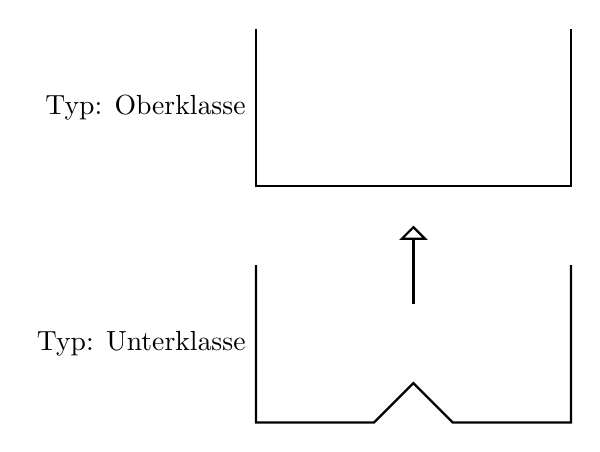
\begin{tikzpicture}
  \draw [thick] (0,3) -- (0, 1) node [left, midway] {Typ: Oberklasse} -- (4,1) -- (4, 3);
  \draw [thick] (0,0) -- (0, -2) node [left, midway] {Typ: Unterklasse} -- (1.5, -2)  -- (2, -1.5) -- (2.5, -2) -- (4,-2) -- (4, 0);
  \draw [thick, open triangle 90-] (2,0.5) -- (2, -0.5);
\end{tikzpicture}

% Oberklasse an Unterklasse 
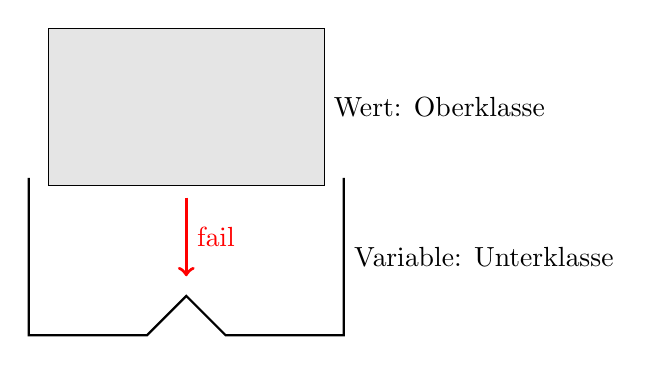
\begin{tikzpicture}
  \filldraw [fill=gray!20] (0.25,2-0.1) -- (0.25, 0-0.1) -- (4-0.25, 0-0.1) -- (4-0.25, 2-0.1)
node [right, midway] {Wert: Oberklasse} -- (0.25,2-0.1) ;
  \draw [thick] (0,0) -- (0, -2) -- (1.5, -2)  -- (2, -1.5) -- (2.5, -2) -- (4,-2) -- (4, 0) node [right, midway] {Variable: Unterklasse};
  \draw [->, very thick, red] (2,-0.25) -- (2,-1.25) node [right, midway, red] {fail};
\end{tikzpicture}

% Unterklasse an Oberklasse 
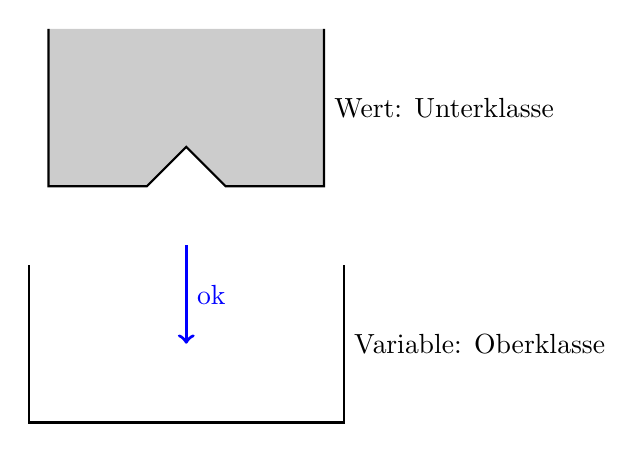
\begin{tikzpicture}
  \filldraw [thick, fill=gray!40] (0.25,3) -- (0.25, 1) -- (1.5, 1)  -- (2, 1.5) -- (2.5, 1) -- (4-0.25,1) -- (4-0.25, 3) node [right, midway] {Wert: Unterklasse};
  \draw [thick] (0,0) -- (0, -2) -- (4,-2) -- (4, 0) node [right, midway] {Variable: Oberklasse};
  \draw [->, very thick, blue] (2,0.25) -- (2,-1) node [right, midway, blue] {ok};
\end{tikzpicture}

% Kleinen Wert an große Variable 
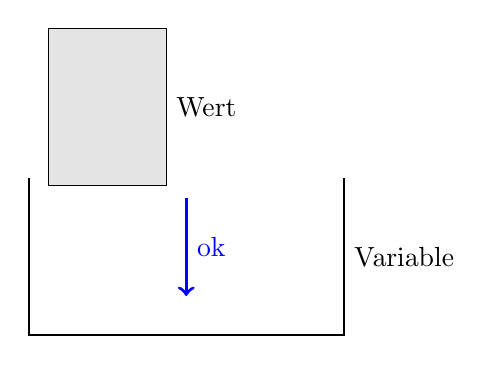
\begin{tikzpicture}
  \draw [thick] (0,0) -- (0, -2) -- (4,-2) -- (4, 0) node [right, midway] {Variable};
  \filldraw [fill=gray!20] (0.25,2-0.1) -- (0.25, 0-0.1) -- (2-0.25, 0-0.1) -- (2-0.25, 2-0.1)
node [right, midway] {Wert} -- (0.25,2-0.1) ;
  \draw [->, very thick, blue] (2,-0.25) -- (2,-1.5) node [right, midway, blue] {ok};
\end{tikzpicture}

% Großer  Wert an kleine  Variable 
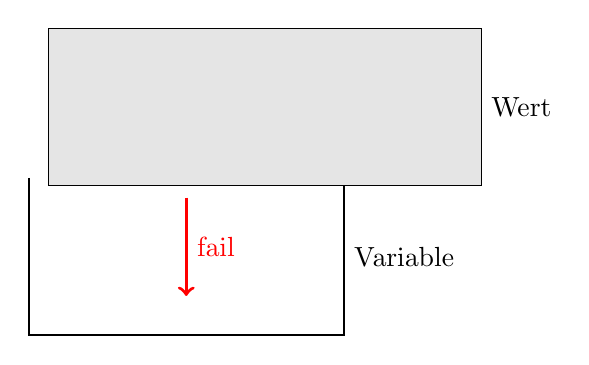
\begin{tikzpicture}
  \draw [thick] (0,0) -- (0, -2) -- (4,-2) -- (4, 0) node [right, midway] {Variable};
  \filldraw [fill=gray!20] (0.25,2-0.1) -- (0.25, 0-0.1) -- (6-0.25, 0-0.1) -- (6-0.25, 2-0.1)
node [right, midway] {Wert} -- (0.25,2-0.1) ;
  \draw [->, very thick, red] (2,-0.25) -- (2,-1.5) node [right, midway, red] {fail};
\end{tikzpicture}


\end{document}